\documentclass[11pt]{article} % use larger type; default would be 10pt
\usepackage[utf8]{inputenc} % set input encoding (not needed with XeLaTeX)

%%% BEGIN Article customizations

%%% PAGE LAYOUT
\usepackage{geometry} % to change the page dimensions
\geometry{a4paper} % or letterpaper (US) or a5paper or....
% \geometry{margin=1in} % for example, change the margins to 2 inches all round
\usepackage[parfill]{parskip} % Activate to begin paragraphs with an empty line rather than an indent

%%% FIGURES
\usepackage{graphicx} % support the \includegraphics command and options
\graphicspath{{../FIGURES/FIGURE_PDFS/}}

%%% PACKAGES
\usepackage{booktabs} % for much better looking tables
\usepackage{array} % for better arrays (eg matrices) in maths
\usepackage{paralist} % very flexible & customisable lists (eg. enumerate/itemize, etc.)
\usepackage{verbatim} % adds environment for commenting out blocks of text & for better verbatim
\usepackage{subfig} % make it possible to include more than one captioned figure/table in a single float
% These packages are all incorporated in the memoir class to one degree or another...

%%% HEADERS & FOOTERS
\usepackage{fancyhdr} % This should be set AFTER setting up the page geometry
\pagestyle{fancy} % options: empty , plain , fancy
\renewcommand{\headrulewidth}{0pt} % customise the layout...
\lhead{}\chead{}\rhead{}
\lfoot{}\cfoot{\thepage}\rfoot{}

%%% SECTION TITLE APPEARANCE
\usepackage{sectsty}
\allsectionsfont{\sffamily\mdseries\upshape} % (See the fntguide.pdf for font help)
% (This matches ConTeXt defaults)

%%% ToC (table of contents) APPEARANCE
\usepackage[nottoc,notlof,notlot]{tocbibind} % Put the bibliography in the ToC
\usepackage[titles,subfigure]{tocloft} % Alter the style of the Table of Contents
\renewcommand{\cftsecfont}{\rmfamily\mdseries\upshape}
\renewcommand{\cftsecpagefont}{\rmfamily\mdseries\upshape} % No bold!

%%% END Article customizations

%%% The "real" document content comes below...

\title{Double Sequencing Analysis (this still needs a title)}
\author{Dakota Z. Derryberry, Claus O. Wilke, Matthew C. Cowperthwaite}

\begin{document}
\maketitle

\section{Introduction}

Intro goes here.

\section{Results}

\subsection{Unfiltered data: WGA v. WGS}

For 55 samples, TCGA has two identical data sets except for the sample preparation: one is whole genome sequencing (WGS) and the other is whole genome amplified sequencing (WGA). We calculated the number of mutations in each of these 110 samples (2 each from 55 patients). The number of mutations per sample ranged considerably, from XX to XX in the WGS samples and from XX to XX in the WGA samples. That the range is higher among the WGA samples is expected, because the amplification process may introduces mutations thereby artificially inflating the number of mutations in the dataset. To test this, we plotted the number of putative SNPs in the WGS and WGA sample preparation for each individual patient. As expected, for most patients, there were more mutations in the WGA sample than in the WGS sample (Figure 1). Surprisingly, not all exceptions had night numbers of mutations. One WGA sample with fewer than 50 mutaions had nearly 500 in the corresponding WGS sample; and one WGS sample with more than 200 mutations had only 200 in the corresponding WGA sample.

\begin{figure}
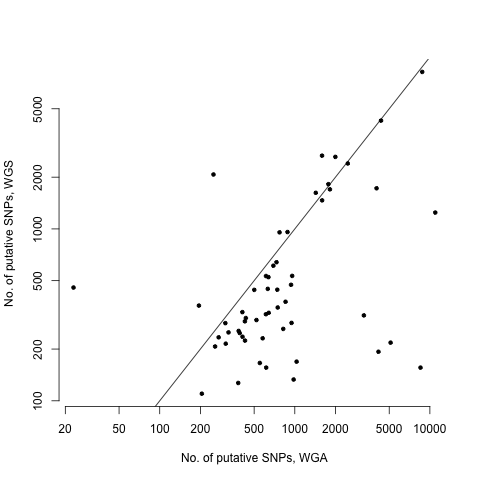
\includegraphics[scale=0.5]{C282_v_C484.png}
\caption{This figure plots the number of putative SNPs called by SomaticSniper (unfiltered) using the WGS v. WGA. Each point is a patient. The line is y=x, so points falling below the line agree with the hypothesis that whole genome amplification makes more mutations in a sample.}
\end{figure}

We next looked at the overlap between the called putative SNPs in the WGS and WGA samples. Although amplification may introduce new mutations, the mutations found in the WGS sample for each patient should be (mostly) a subset of those found in the WGA sample for that same patient. Although WGS may itself introduce some new mutations, the percent of WGS mutations that overlap with those found in the WGA sample should be significantly higher than the percent of WGA mutations found in the overlap with WGS. To test this, we calculated the overlap between the WGS and WGA samples for each patient. As expected, WGS samples have fewer non-overlapping putative SNPs than WGA samples (Figure 2). 

\begin{figure}
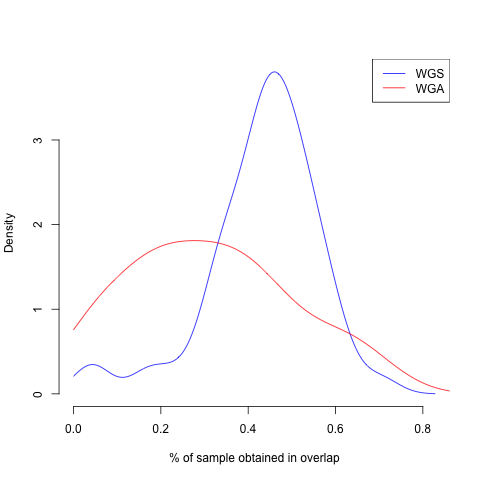
\includegraphics[scale=0.5]{unfiltered_overlap_WGS_WGA_together_densities.png}
\caption{This figure shows the density of the percentage of each WGS (blue) and WGA (red) sample that overlaps with the other from teh same patient. The WGS distribution is higher and narrower, showing that the WGS samples overall have a higher percentage overlap than the WGA samples, and less range in this parameter. }
\end{figure}

Although most samples agree with the hypotheses in figures one and two, there are outlyers: 

\begin{figure}
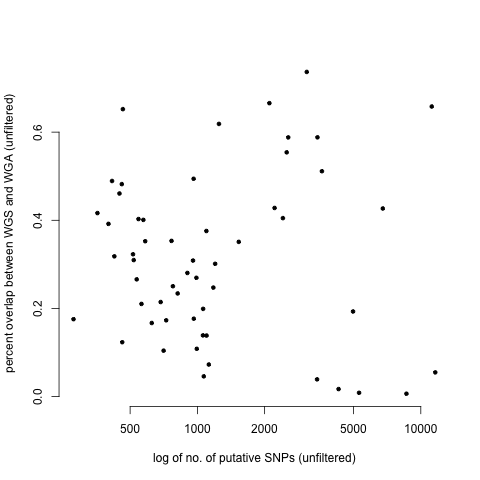
\includegraphics[scale=0.5]{unfiltered_total_muts_v_percent_overlap.png}
\caption{This is figure 3}
\end{figure}

\subsection{Unfiltered data: Time points}

\subsection{Filtering}

\section{Methods}

\subsection{Data and back-end processing}

All sequence data came from The Cancer Genome Atlas (TCGA) Gliobastoma multiforme (GBM) data set. We downloaded raw reads in (XXX format) using (CGHub?) on (date) for 68 patients. For each patient, data consisted of one set of rads taken from blood DNA, and two sets of reads taken from tumor DNA. In 55 cases, the two sets of reads from tumor DNA were one set of reads from whole genome sequencing (WGS) and one set of reads from whole genome sequencing with amplification (WGA). In 13 cases, the two sets of reads from tumor DNA were one set of reads pre-readiation treatment and one set post-radiation treatment. We developed a pipeline to align all reads to HG19. This pipeline used (bowtie?) for alignment and (bedtools? whatever -- quality control...) We used SomaticSniper to align each tumor sequence with it's corresponding blood sequence. We then filtered the SomaticSniper data using 8 custom filters. These removed (i) , (ii) , (iii) , (iv) , (v) , (vi) , (vii) , and (viii) . All custom code is available in a github repository, located at (webaddress). In addition to sequence data, filter 6 uses dbSNP, version 137, to find common SNPs among the putative mutaitons called by SomaticSniper.

\subsection{Analysis}

We used custom python scripts, available in the above github repository, to perform simple calculations and data operations. We used R to do statistics and generate figures, and this code is also availabel in the git repository.  

\section{Discussion}

What do I think of this?

\end{document}
